\documentclass{standalone}
\usepackage{tikz}

\begin{document}
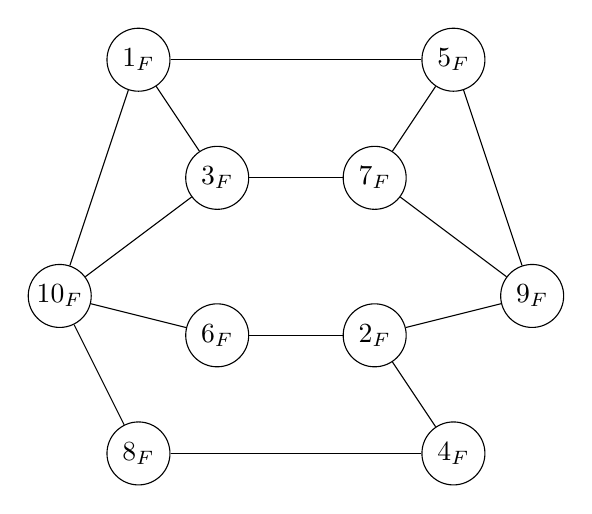
\begin{tikzpicture}[
    every node/.style={circle, draw, minimum size=0.8cm, inner sep=1pt}
]

\node (1) at (0,3) {$1_F$};
\node (5) at (4,3) {$5_F$};
\node (3) at (1,1.5) {$3_F$};
\node (7) at (3,1.5) {$7_F$};
\node (10) at (-1,0) {$10_F$};
\node (6) at (1,-0.5) {$6_F$};
\node (2) at (3,-0.5) {$2_F$};
\node (9) at (5,0) {$9_F$};
\node (8) at (0,-2) {$8_F$};
\node (4) at (4,-2) {$4_F$};

\draw (1) -- (5);
\draw (1) -- (3);
\draw (1) -- (10);
\draw (5) -- (7);
\draw (5) -- (9);
\draw (3) -- (7);
\draw (10) -- (3);
\draw (7) -- (9);
\draw (10) -- (6);
\draw (10) -- (8);
\draw (6) -- (2);
\draw (2) -- (9);
\draw (2) -- (4);
\draw (8) -- (4);

\end{tikzpicture}
\end{document}